\paragraph{QuizziPedia::Back-End::App::Controllers::ErrorsHandler}
\begin{figure}[ht]
	\centering
	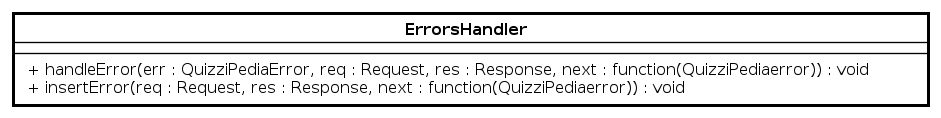
\includegraphics[scale=0.6]{UML/Classi/Back-End/QuizziPedia_Back-End_App_Controllers_ErrorsHandler.png}
	\caption{QuizziPedia::Back-End::App::Controllers::ErrorsHandler}
\end{figure}
\FloatBarrier


\begin{itemize}
	\item \textbf{Descrizione}:
	classe \textit{middleware\ped{G}} per la gestione degli errori. Ritorna al client un oggetto di tipo \texttt{Response} con stato \textit{HTTP\ped{G}} 500 e descrizione dell'errore in formato \textit{JSON\ped{G}}. È un componente \textit{ConcreteHandler\ped{G}} del \textit{design pattern\ped{G}} \textit{Chain of responsibility\ped{G}};
	\item \textbf{Utilizzo}:
	viene utilizzata quando si verifica un errore. Si preoccupa di delegare la costruzione del messaggio d'errore al modulo specifico qualora questo esista, altrimenti costruisce un messaggio d'errore generico. In questo modo i messaggi d'errore specifici vengono delegati ad un altro modulo, rendendo così possibile aggiungere in futuro altri moduli per gestire più flessibilmente nuove tipologie di errori;
	\item \textbf{Relazioni con altre classi}:
	\begin{itemize}
		\item \textbf{IN \texttt{QuizRouter}}:
		classe che gestisce le richieste relative alla gestione di un questionario. Componente \textit{ConcreteHandler\ped{G}} del \textit{design pattern\ped{G}} \textit{Chain of responsibility\ped{G}};
		\item \textbf{IN \texttt{QuestionRouter}}:
		classe che gestisce le richieste relative alla gestione di una domanda. Componente \textit{ConcreteHandler\ped{G}} del \textit{design pattern\ped{G}} \textit{Chain of responsibility\ped{G}};
		\item \textbf{IN \texttt{UserRouter}}:
		classe che gestisce le richieste relative alla gestione di un utente. Componente \textit{ConcreteHandler\ped{G}} del \textit{design pattern\ped{G}} \textit{Chain of responsibility\ped{G}}; Utilizza il modulo \textit{Passport\ped{G}};
		\item \textbf{OUT \texttt{QuizziPediaError}}:
		classe di gestione degli errori. Esegue la costruzione del messaggio d'errore specifico per i moduli di QuizziPedia::Back-End::App.
	\end{itemize}
	\item \textbf{Metodi}:
	\begin{itemize}
		\item \texttt{+ handleError(err: QuizziPediaError, req: Request, res: Response, \\next: function(QuizziPediaError)):void}\\
		Metodo che gestisce la costruzione dei messaggi d'errore ritornando un \textit{JSON\ped{G}} contenente il messaggio d'errore.\\
		\textbf{Parametri}:
		\begin{itemize}
			\item \texttt{err: QuizziPediaError}\\
			Rappresenta l'errore di tipo \texttt{QuizziPediaError};
			\item \texttt{req: Request}\\
			Rappresenta la richiesta inviata al \textit{server\ped{G}};
			\item \texttt{res: Response}\\
			Rappresenta la risposta che il \textit{server\ped{G}} fornirà al termine dell'esecuzione del metodo;
			\item \texttt{next: function(QuizziPediaError)}\\
			Rappresenta la \textit{callback\ped{G}} che il metodo deve chiamare al termine dell'elaborazione per passare il controllo ai successivi \textit{middleware\ped{G}}. La presenza del parametro facoltativo \texttt{QuizziPediaError} attiva la catena di gestione dell'errore in sostituzione della normale catena di gestione delle richieste.
		\end{itemize}
	\end{itemize}
\end{itemize}
